\documentclass[11pt,letterpaper]{article}
\usepackage[lmargin=1in,rmargin=1in,tmargin=1in,bmargin=1in]{geometry}
\usepackage{../style/homework}
\usepackage{../style/commands}
\setbool{quotetype}{true} % True: Side; False: Under
\setbool{hideans}{false} % Student: True; Instructor: False

% -------------------
% Content
% -------------------
\begin{document}

\homework{2: Due 02/14}{Whatcha got there? Numbers?}{Bender Bending Rodriguez, Futurama}

% Problem 1
\problem{10} Tyrell sells mattresses in a store which he rents for \$7500 per month with building costs of approximately \$635 per month. He purchases these mattresses from a distributor at an average cost of \$127 per mattress. On average, each mattress sells for \$547.
        \begin{enumerate}[(a)]
        \item What are Tyrell's fixed costs?
        \item Find $C(m)$, the cost function associated to selling $m$ mattresses. 
        \item Find $R(m)$, the revenue function function for selling $m$ mattresses. 
        \item Without finding $P(m)$, the profit function, find the minimum number of mattresses Tyrell needs to sell each month to make a profit. 
        \end{enumerate} \pspace

\sol
\begin{enumerate}[(a)]
\item The fixed costs are the costs not associated with production. The fixed costs here are the rent, which is \$7500. 

\item We know that $C(x)= \text{FC} + \text{VC}$. We know from (a) that the fixed costs are 7500. Each mattress costs \$127. Therefore, if Tyrell buys $x$ mattresses, he spends $127x$. This is the variable cost, VC. Therefore, we have\dots
	\[
	C(x)= 127x + 7500
	\]

\item We know that each mattress sells for roughly \$547. Therefore, if $x$ mattresses are sold, the revenue is $547x$. Then we must have\dots
	\[
	R(x)= 547x 
	\]

\item We know that the profit is the revenue minus the cost. Therefore,
	\[
	\begin{aligned}
	P(x)&= R(x) - C(x) \\[0.3cm]
	&= 547x - (127x + 7500) \\[0.3cm]
	&= 547x - 127x - 7500 \\[0.3cm]
	&= 420x - 7500
	\end{aligned}
	\]
Furthermore, because $P(x)$ is linear, we know that we will make a profit for $x$ values greater than the breakeven point---which occurs when $P(x)= 0$. But then\dots
	\[
	\begin{aligned}
	P(x)&= 0 \\[0.3cm]
	420x - 7500&= 0 \\[0.3cm]
	420x&= 7500 \\[0.3cm]
	x&\approx 17.86
	\end{aligned}
	\]
Therefore, 18~mattresses need to be sold to make a profit. 
\end{enumerate}



\newpage



% Problem 2
\problem{10} Cheesy Does It is a cheese shop which sells a large variety of cheeses. Suppose they order gouda cheese from a local distributor at a rate of \$5.83 per pound (lb). They are charged a delivery fee of \$87.25 per order. To make a profit selling this cheese, they markup their purchased price by 60\%. 
	\begin{enumerate}[(a)]
	\item Find $C(\ell)$, the costs associated with selling $\ell$ pounds of gouda cheese.
	\item Find $R(\ell)$, the revenue associated with selling $\ell$ pounds of gouda cheese.
	\item Find $P(\ell)$, the profit associated with selling $\ell$ pounds of gouda cheese.
	\item Using $P(\ell)$, find the minimum number of pounds of gouda cheese the store must sell to turn a profit on these cheese sales. 
	\end{enumerate} \pspace

\sol
\begin{enumerate}[(a)]
\item We know that $C(\ell)= \text{FC} + \text{VC}$. The fixed costs, FC, is the delivery cost for the cheese, which is \$87.25. Because the cheese costs \$5.83 per pound, if $\ell$ pounds are purchased, the total price is $5.83\ell$. But then we know that the variable costs are $5.83\ell$. Therefore, 
	\[
	C(\ell)= 5.83\ell + 87.25
	\]

\item The cheese costs \$5.83 per pound. To make a profit, the shop marks this up by 60\%. But then the cost of the cheese is $5.83(1 + 0.60)= 5.83(1.60)= 9.33$. If $\ell$ pounds are purchased, then the revenue is $9.33\ell$. Therefore,
	\[
	R(\ell)= 9.33\ell
	\]

\item We know that the profit function is the revenue function minus the cost function. Therefore,
	\[
	\begin{aligned}
	P(\ell)&= R(\ell) - C(\ell) \\[0.3cm]
	&= 9.33\ell - (5.83\ell + 87.25) \\[0.3cm]
	&= 9.33\ell - 5.83 \ell - 87.25 \\[0.3cm]
	&= 3.50\ell - 87.25
	\end{aligned}
	\]

\item Because $P(\ell)$ is linear, we know that we will make a profit for $\ell$ values greater than the breakeven point---which occurs when $P(\ell)= 0$. But then\dots
	\[
	\begin{aligned}
	P(\ell)&= 0 \\[0.3cm]
	3.50\ell - 87.25&= 0 \\[0.3cm]
	3.50\ell&= 87.25 \\[0.3cm]
	\ell&\approx 24.93
	\end{aligned}
	\]
Therefore, 25~pounds of cheese need to be sold to make a profit. 
\end{enumerate}



\newpage



% Problem 3
\problem{10} Suppose you have profit and cost functions given by $R(x)= 95.55x$ and $C(x)= 24.35x + 11450$, respectively. 
	\begin{enumerate}[(a)]
	\item How much does each item sell for? Explain how you know.
	\item What are the fixed costs? Explain how you know.
	\item Find the revenue and costs associated to selling 120~items. Is the seller making a profit?
	\item Sketch $R(x)$, $C(x)$, and $P(x)$ (the profit function) on the same graph---being sure to include the equilibrium point. 
	\end{enumerate} \pspace

\sol
\begin{enumerate}[(a)]
\item Observe that $R(x)$ and $C(x)$ are linear. But then the purchased price is the slope of $C(x)$, which is 24.35. Therefore, the vendor purchases the item for \$24.35 per item. The slope of $R(x)$ is the sale price of the item. The slope of $R(x)$ is 95.55. Therefore, the item sells for \$95.55 per item. 

\item The fixed costs are the costs incurred regardless of production. Therefore, the fixed costs should be the costs when $x= 0$. But then we have\dots
	\[
	C(0)= 24.35(0) + 11450= 0 + 11450= 11450 
	\] 
Therefore, the fixed costs are \$11,450. 

\item We evaluate $R(x)$ and $C(x)$ at $x= 120$:
	\[
	\begin{aligned}
	R(120)&= 95.55(120)= 11466 \\
	C(120)&= 24.35(120) + 11450= 2922 + 11450= 14372
	\end{aligned}
	\]
Therefore, the revenue for selling 120~items is \$11,466 and the costs are \$14,372. Because $R(120) < C(120)$, we know that there is a loss---not a profit. 

\item Note that $P(x)= R(x) - C(x)= 71.20x - 11450$. Setting this equal to zero, we find that $x= 160.815$. Therefore, the breakeven point occurs when $x= 160.815$, where $R(160.815) \approx 15366$ and $C(160.815)= 15366$. Then we have the following plot (with the $y$-axis in hundreds of dollars):
	\[
	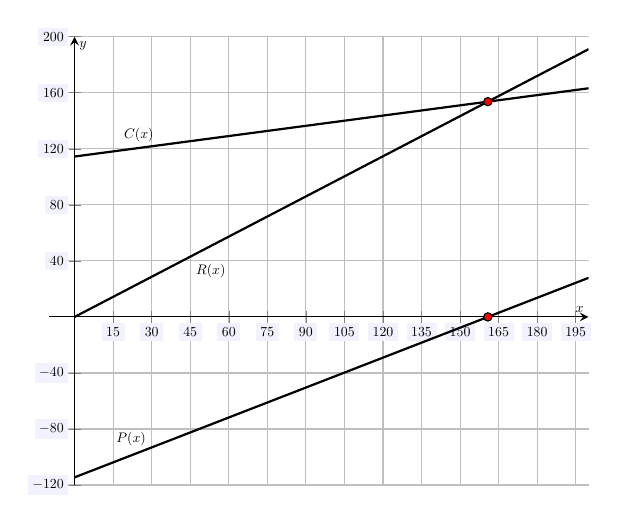
\begin{tikzpicture}[scale=1,every node/.style={scale=0.5}]
	\begin{axis}[
	grid=both,
	axis lines=middle,
	ticklabel style={fill=blue!5!white},
	xmin= -10, xmax=200,
	ymin= -120, ymax=200,
	xtick={0,15,...,200},
	ytick={-120,-80,...,200},
	xlabel=\(x\),ylabel=\(y\),
	]
	\addplot[thick, domain= 0:200] {0.9555*x};
	\addplot[thick, domain= 0:200] {0.2435*x + 114.5};
	\addplot[thick, domain= 0:200] {0.7120*x - 114.50};
	\node at (25,130) {$C(x)$};
	\node at (53,33) {$R(x)$};
	\node at (22,-87) {$P(x)$};
	
	\draw[fill=red] (160.815,153.66) circle (1.5pt);
	\draw[fill=red] (160.815,0) circle (1.5pt);
	\end{axis}
	\end{tikzpicture}
	\]
\end{enumerate}



\newpage



% Problem 4
\problem{10} Suppose the barbershop Jack the Clipper has a revenue function and cost functions $R(x)= 0.04x^2 + 23x - 15$ and $C(x)= 5.2x + 3100$, respectively, where $x$ is the number of haircuts given. 
	\begin{enumerate}[(a)]
	\item Find the average revenue, cost, and profit for giving 160 haircuts.
	\item Find the marginal revenue, cost, and profit for giving 160 haircuts. 
	\end{enumerate} \pspace

\sol
\begin{enumerate}[(a)]
\item First, observe that\dots
	\[
	\begin{aligned}
	R(160)&= 0.04(160)^2 + 23(160) - 15= 1024 + 3680 - 15= 4689 \\
	C(160)&= 5.2(160) + 3100= 832 + 3100= 3932
	\end{aligned}
	\]
Then $P(160)= R(160) - C(160)= 4689 - 3932= 757$. Then we have\dots
	\[
	\begin{aligned}
	\text{Avg. }R(160)&= \dfrac{4689}{160} \approx 29.31 \\
	\text{Avg. }C(160)&= \dfrac{3932}{160} \approx 24.58 \\
	\text{Avg. }P(160)&= \dfrac{757}{160} \approx 4.73
	\end{aligned}
	\] \pspace

\item Observe that we also have\dots
	\[
	\begin{aligned}
	R(161)&= 0.04(161)^2 + 23(161) - 15= 1036.84 + 3703 - 15= 4724.84 \\
	C(161)&= 5.2(161) + 3100= 837.20 + 3100= 3937.20
	\end{aligned}
	\]
Then $P(161)= R(161) - C(161)= 4724.84 - 3937.20= 787.64$. Then we have\dots
	\[
	\begin{aligned}
	\text{Marg. }R(160)&= R(161) - R(160)= 4724.84 - 4689= 35.84 \\
	\text{Marg. }C(160)&= C(161) - C(160)= 3937.20 - 3932= 5.20 \\
	\text{Marg. }P(160)&= P(161) - P(160)= 787.64 - 757= 30.64
	\end{aligned}
	\]
\end{enumerate}



\newpage



% Problem 5
\problem{10} Spruce Springclean is a cleaning company which offers a basic and deluxe package. The revenue function for $b$ basic cleanings and $d$ deluxe cleanings is $R(b, d)= 45.99b + 69.99d$, while the associated cost function is $C(b, d)= 5.45b + 8.11d + 7.5$. 
	\begin{enumerate}[(a)]
	\item How much does a basic and deluxe cleaning cost? Explain how you know. 
	\item Find the fixed costs.
	\item Find the costs, revenue, and profit for performing 34 basic cleanings and 29 deluxe cleanings. 
	\end{enumerate} \pspace

\sol
\begin{enumerate}[(a)]
\item Because $R(b, d)$ and $C(b, d)$ are (affine) linear functions, we know that the costs are the `slopes' in each `direction.' Therefore examining $C(b, d)$, the cost for the company for a basic cleaning is \$5.45 per cleaning and the cost of a deluxe cleaning is \$8.11 per cleaning. Examining $R(b, d)$, the company charges \$45.99 per basic cleaning and \$69.99 per deluxe cleaning. \pspace

\item The fixed costs are the costs incurred regardless of production. Therefore, the fixed costs should be $C(b, d)$ when $b= 0$ and $d= 0$. But then we have\dots
	\[
	C(0, 0)= 5.45(0) + 8.11(0) + 7.5= 0 + 0 + 7.5= 7.5
	\]
Therefore, the fixed costs are \$7.50. \pspace

\item We know that $P(b, d)= R(b, d) - C(b, d)$. But then we have\dots
	\[
	\begin{aligned}
	P(b, d)&= R(b, d) - C(b, d) \\
	&= (45.99b + 69.99d) - (5.45b + 8.11d + 7.5) \\
	&= 45.99b + 69.99d - 5.45b - 8.11d - 7.5 \\
	&= 40.54b + 61.88d - 7.5
	\end{aligned}
	\] 
To find the costs, revenue, and profit for performing 34 basic cleanings and 29 deluxe cleanings, we evaluate at $b= 34$ and $d= 29$:
	\[
	\begin{aligned}
	C(34, 29)&= 5.45(34) + 8.11(29) + 7.5= 185.30 + 235.19 + 7.5= 427.99 \\
	R(34, 29)&= 45.99(34) + 69.99(29)= 1563.66 + 2029.71= 3593.37 \\
	P(34, 29)&= 40.54(34) + 61.88(29) - 7.5= 1378.36 + 1794.52 - 7.5= 3165.38
	\end{aligned}
	\] 
\end{enumerate}


\end{document}